\documentclass[12pt, a4paper]{article}
\usepackage{cmap} % Улучшенный поиск русских слов в полученном pdf-файле
\usepackage[T2A]{fontenc} % Поддержка русских букв
\usepackage[utf8]{inputenc} % Кодировка utf8
\usepackage[english, russian]{babel} % Языки: русский, английский

\usepackage{enumitem}
\usepackage{multicol}
\usepackage{pscyr} % Нормальные шрифты

\usepackage{amsmath}
\usepackage{amsthm}
\usepackage{amssymb}

\usepackage{fancyhdr}
\usepackage{titling}
\usepackage{indentfirst}
\usepackage{cancel}
\usepackage{soulutf8}
\usepackage{wrapfig}
\usepackage{gensymb}
\usepackage[dvipsnames,table,xcdraw]{xcolor}
\usepackage{graphbox}
\usepackage{tikz}
\usepackage{pgfplots}
\usepackage{mathrsfs}
\usetikzlibrary{positioning}
%Русские символы в списке
\makeatletter
\AddEnumerateCounter{\asbuk}{\russian@alph}{щ}
\makeatother

\usepackage{graphicx}
\graphicspath{{pic/}}
\DeclareGraphicsExtensions{.pdf,.png,.jpg}

%Изменеие параметров листа
\usepackage[left=15mm,right=15mm,
top=2cm,bottom=2cm,bindingoffset=0cm]{geometry}

\pagestyle{fancy}
\setlength\parindent{1,5em}

\pgfplotsset{
	width=10cm,
	compat=newest,
	every axis/.append style={
		axis x line=middle,
		axis y line=middle,
		unit vector ratio = 1 1,
		xlabel={$x$},
		xlabel style={below left},
		ylabel={$y$},
		ylabel style={below left},
		ymajorgrids=true,
		xmajorgrids=true,
		xticklabels={},
		yticklabels={},
		samples=1000,
		grid=both,
		grid style={thick},
		very thick,
		ticks=both,
		xtick={-100,-99,...,100},
		ytick={-100,-99,...,100},
		restrict y to domain=--100:100
}}

\begin{document}
		
\lhead{Функции}
\rhead{Школа <<Симметрия>>}

\section{Параболы}
\begin{enumerate}
	\item
	\begin{minipage}[t][8cm][t]{0.5\textwidth}
		На рисунке изображен график функции вида $y=ax^2+bx+c$, где числа $a$, $b$ и $c$ — целые. Вычислите $f\left(\dfrac{1}{4}\right)-f\left(\dfrac{1}{2}\right)$.
		\begin{flushright}
			\rotatebox{180}{\fbox{$-0,3125$}}
		\end{flushright}
	\end{minipage}
	\begin{minipage}[t][8cm][t]{0.5\textwidth}
		\hspace{10pt}
		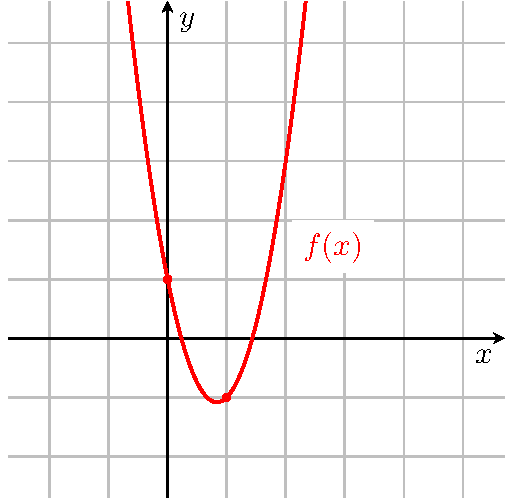
\includegraphics[align=t, width=0.8\textwidth]{graphs/graph_1/graph_1}
	\end{minipage}
\end{enumerate}
\section{Гиперболы}
\begin{enumerate}
	\item 
	\begin{minipage}[t][8cm][t]{0.5\textwidth}
		На рисунке изображен график функции вида $y=\dfrac{a}{x+b}+c$, где числа $a$, $b$ и $c$ — целые. Найдите $f\left(-\dfrac{8}{5}\right)$.
		\begin{flushright}
			\rotatebox{180}{\fbox{$-1\dfrac{1}{3}$}}
		\end{flushright}
	\end{minipage}
	\begin{minipage}[t][8cm][t]{0.5\textwidth}
		\hspace{10pt}
		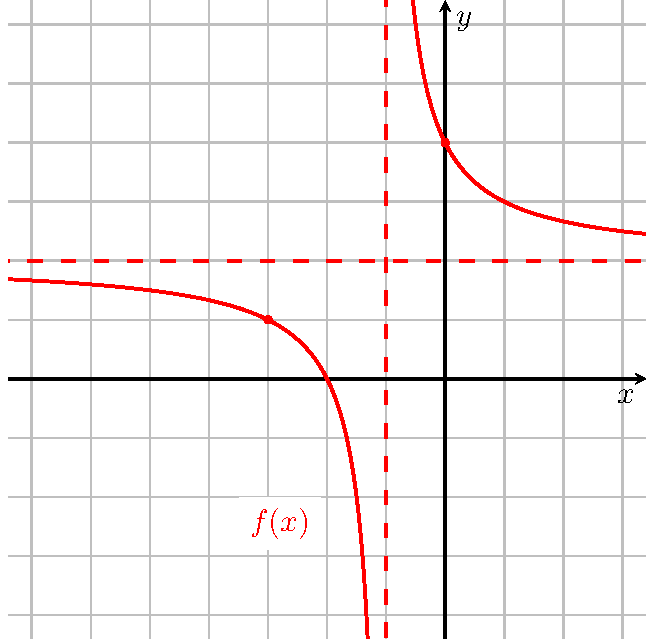
\includegraphics[align=t, width=0.8\textwidth]{graphs/graph_2/graph_2}
	\end{minipage}
	
\end{enumerate}
\end{document}